\documentclass[10pt]{article}
\usepackage[portuguese]{babel}
\usepackage[utf8]{inputenc}
\usepackage[pdftex]{graphicx}
\usepackage{venndiagram}
\usepackage{subcaption}
\usepackage{caption}
\usepackage[backend=biber,style=authoryear-ibid]{biblatex}
\usepackage[normalem]{ulem}
\usepackage[margin=0.8in]{geometry}
%\addbibresource{}
\graphicspath{{Pictures/}}
\usepackage{tikz}
\usepackage{setspace}
\usepackage{enumitem}
\usepackage{textcomp}
\usepackage{listings}
\usepackage{float}


\author{}
\title{}
\date{}

\newcommand{\quotebox}[3]{
  \begin{center}
\noindent\fbox{ 
  \parbox{#3\textwidth}{%
  {\itshape#1\itshape}

  \raggedleft {\textbf{#2}} 
    }%  
}
\end{center}
}

\newcommand{\spawnfig}[3]
{
  \begin{figure}[h]
  \centering
  \includegraphics[scale={#3}]{#1}
  \caption{#2}
  \end{figure}
}


\begin{document}
\maketitle

\section{Program Scope}

The program should be able to receive as input a chess move in UCI(Universal
Chess Interface) format i.e
e2e4, and if the movement is valid, output the board state to the user or inform
the user the input isn't valid. For this matter, the standard python library is
enough address the problem. For debugging purposes, a graphical interface was
also required and implemented in pygame, a graphical framework for games.


\section{Program project}

\begin{figure}[H]
    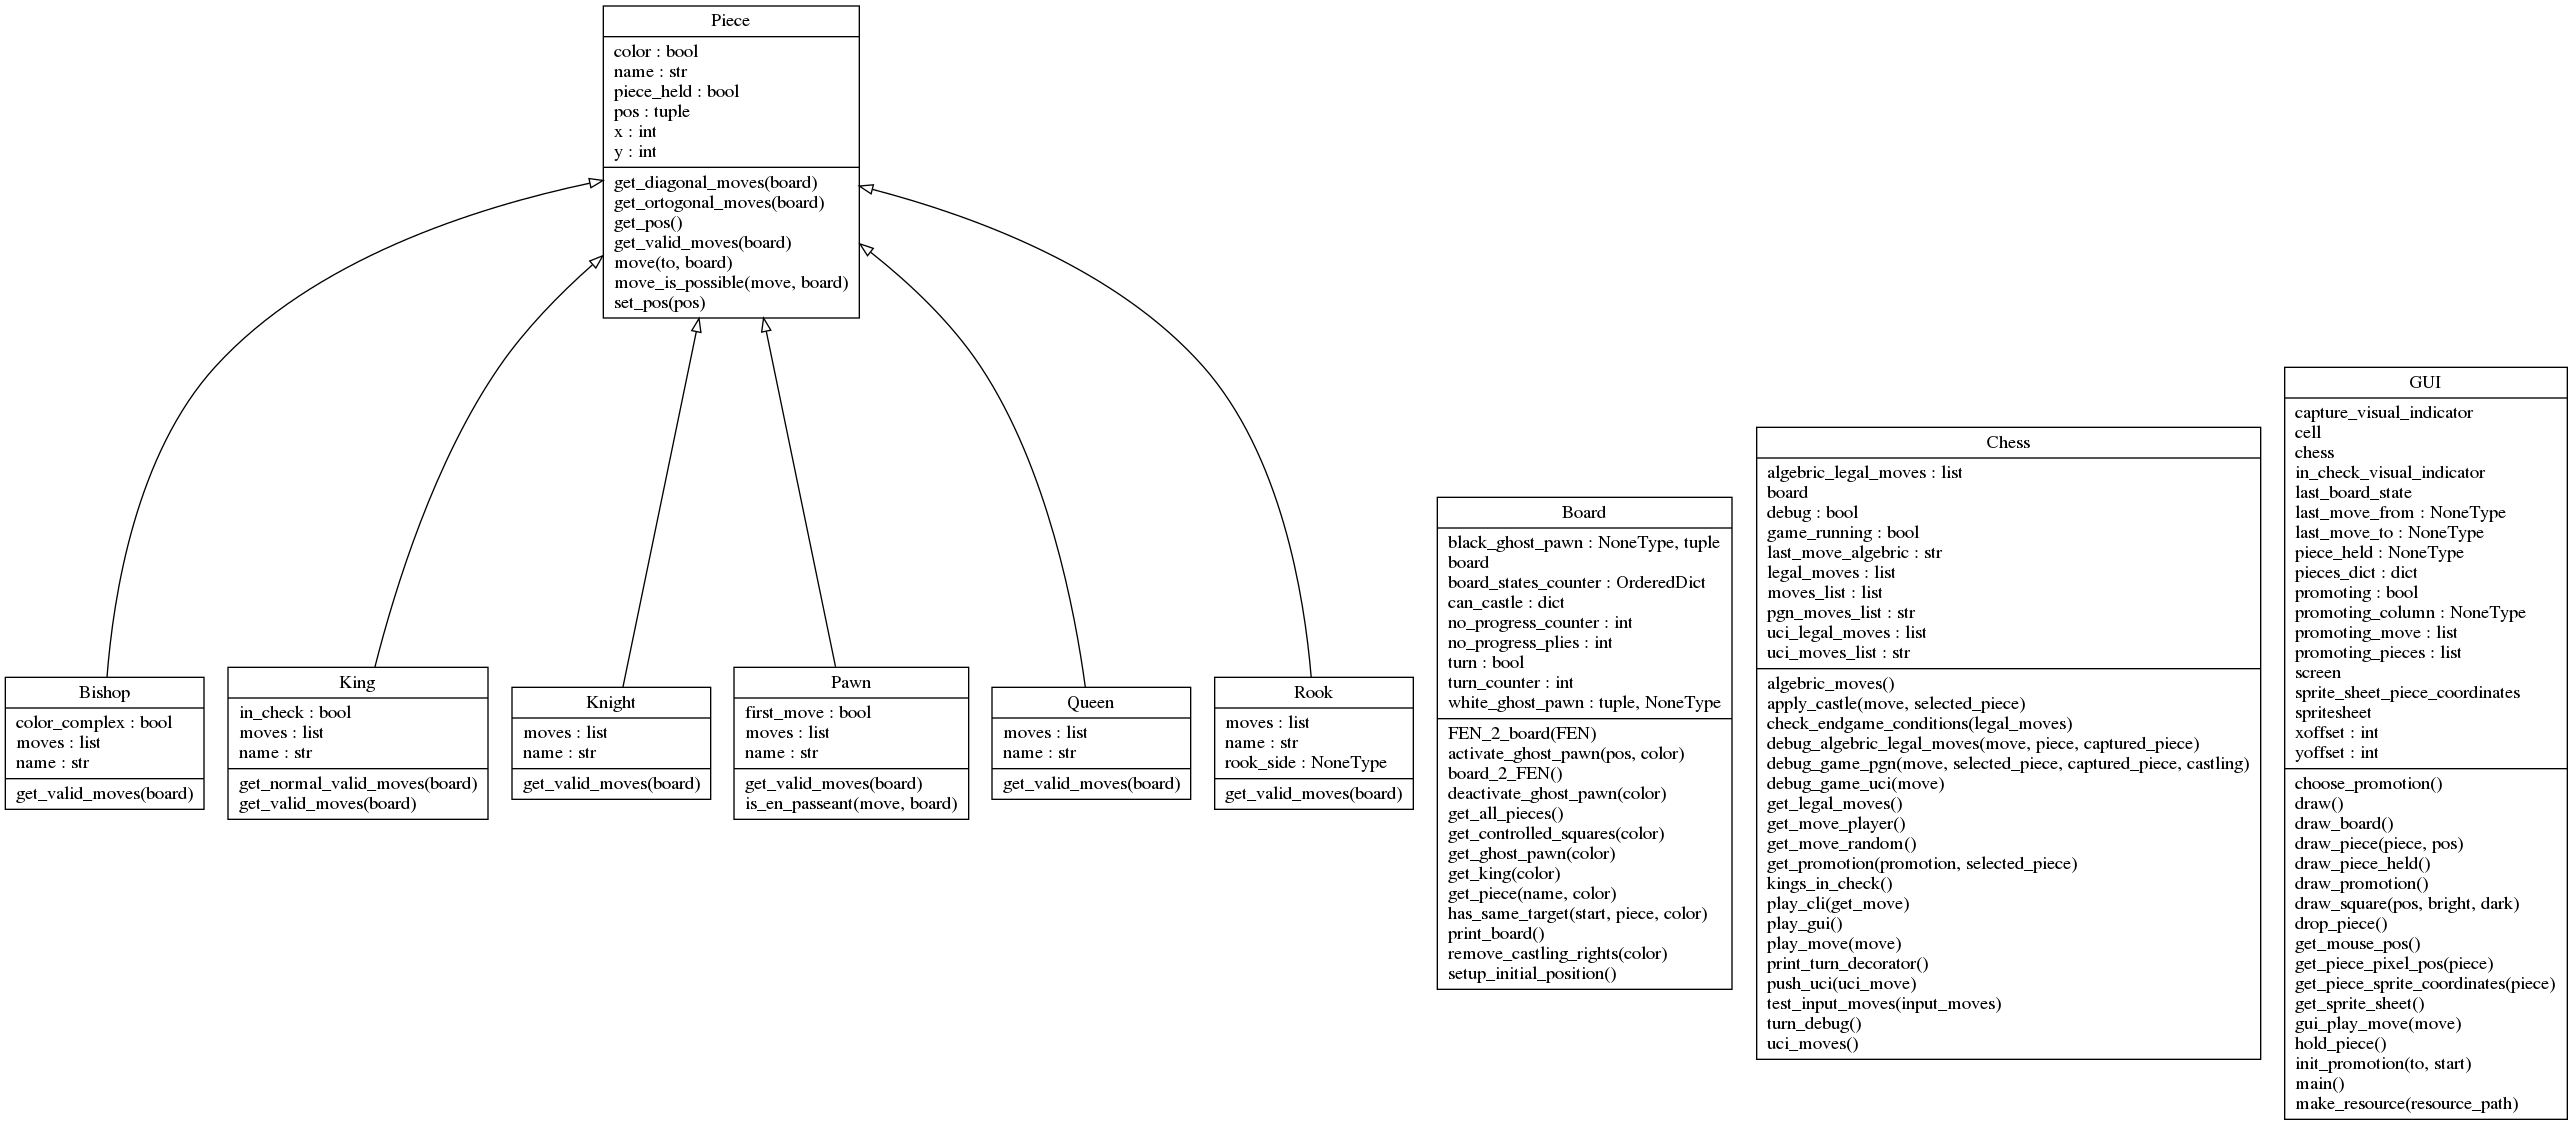
\includegraphics[scale=0.2]{fig/classes_Chess.png}
\end{figure}


\section{Testing}

\begin{table}[h]
\center
\begin{tabular}{|c|c|}
\hline
\textbf{Number of plies (half-moves)}  & \textbf{Number of possible games}  \\
\hline
  1   & 20 \\
\hline
   2  &  400 \\
\hline
  3   & 8092 \\
\hline
4  & 197,281 \\
\hline
5   & 4,865,609 \\
\hline
6   & 119,060,324 \\
\hline
\ldots & \ldots \\
\hline
10 & 69,352,859,712,417 \\
\hline
\end{tabular}
\caption{Shannon's Calculation. Obs: A turn is composed by a white move and a black move. Five plies
therefore stands for white playing three times and black two.}
\end{table}

For testing the general accuracy of the game, it was used the Shannon Number,
which stands for all the possible moves that can be played until a certain
ply(half-move). By the limitation of the computer power avaible for our
disposal, and considering that the game was not written in a language nor
written in a way for fast computation, we could only check the precision of the
game until 5 ply, as we can see by the test log:
\begin{lstlisting}
2022-01-22 00:00:36,742 Result of possible games with 1 ply: 20/20 - OK
2022-01-22 00:00:36,742 Elapsed time in 1 ply: 00h00m00s seconds
2022-01-22 00:00:37,312 Result of possible games with 2 ply: 400/400 - OK
2022-01-22 00:00:37,312 Elapsed time in 2 ply: 00h00m00s seconds
2022-01-22 00:00:52,137 Result of possible games with 3 ply: 8902/8902 - OK
2022-01-22 00:00:52,137 Elapsed time in 3 ply: 00h00m14s seconds
2022-01-22 00:07:11,715 Result of possible games with 4 ply: 197281/197281 - OK
2022-01-22 00:07:11,715 Elapsed time in 4 ply: 00h06m19s seconds
2022-01-22 08:45:00,073 Result of possible games with 5 ply: 4865609/4865609 - OK
2022-01-22 08:45:00,073 Elapsed time in 5 ply: 08h37m48s seconds
    
\end{lstlisting}

Although this is a good signal that basic operations are working, in 5 plies we
cannot test all the complications that might arise during a chess game.

\begin{table}[h]
\center
\begin{tabular}{|c|c|c|c|c|c|c|c|c|}
\hline
\textbf{Depth}   & \textbf{Captures} & \textbf{E.P} &
\textbf{Castles} & \textbf{Promotions} & \textbf{Checks} & \textbf{Dscry
Checks} & \textbf{Dbl Checks} & \textbf{Checkmates} \\
\hline
   1  & 0 & 0 & 0 & 0 & 0 & 0 & 0 & 0 \\
\hline
   2  & 0 & 0 & 0 & 0 & 0 & 0 & 0 & 0 \\
\hline
   3  & 34 & 0 & 0 & 0 & 12 & 0 & 0 & 0 \\
\hline
   4  & 1576 & 0 & 0 & 0 & 469 & 0 & 0 & 8 \\
\hline
5  & 82,719 & 258 & 0 & 0 & 27,251 & 6 & 0 & 347 \\
\hline
\end{tabular}
\caption{Number of ``special'' moves by depth accordingly to
\url{https://www.chessprogramming.org/Perft_Results} }
\end{table}

By this table we can see that we need to concentrate our efforts in testing
Castle, Promotions, Discovery Checks and Double Checks

Specific tests were also made when debugging certain problems in code. So it was
possible to replay a certain game until a specific move and debug it from there,
without manually giving the moves as input.

For example, at 5 ply, there can't be a game with a promoted pawn case,
therefore we need to make a specific test case for that matter. 
\begin{lstlisting}
python3 tests/promotionTest.py
python3 chess.py -guitest g2g4 h7h5 g4h5 g7g6  h5h6  h8h7  f2f3  h7g7  h6h7  f7f6 
... 
PlayedMoves: 1. g4 h5 2. gxh5 g6 3. h6 Rh7 4. f3 Rg7 5. h7 f6 
\end{lstlisting}

\begin{figure}[H]
    \center
    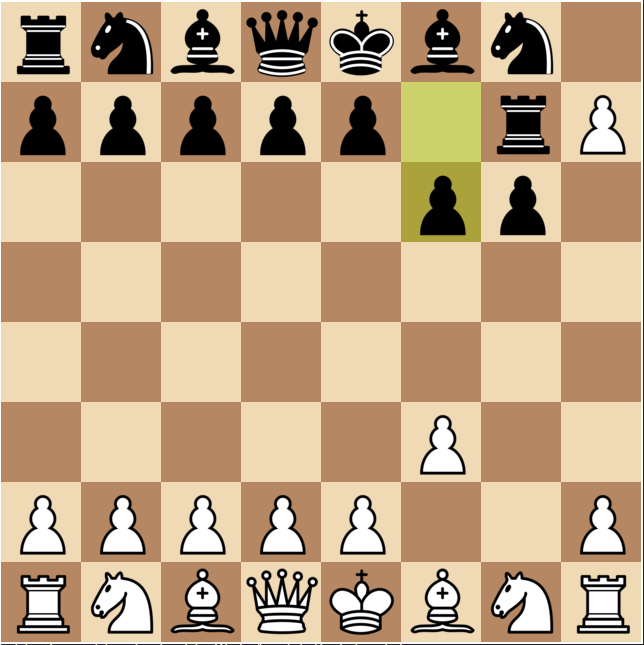
\includegraphics[scale=0.15]{{fig/pre_promotion.png}}
    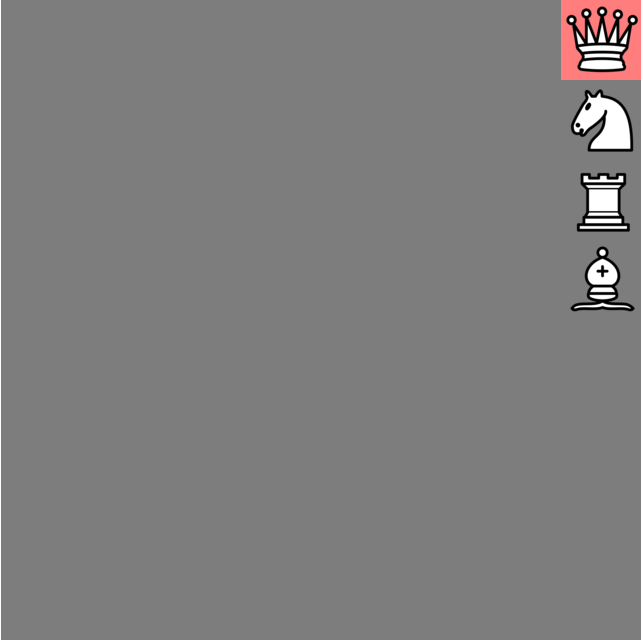
\includegraphics[scale=0.15]{{fig/promoting_pawn.png}}
    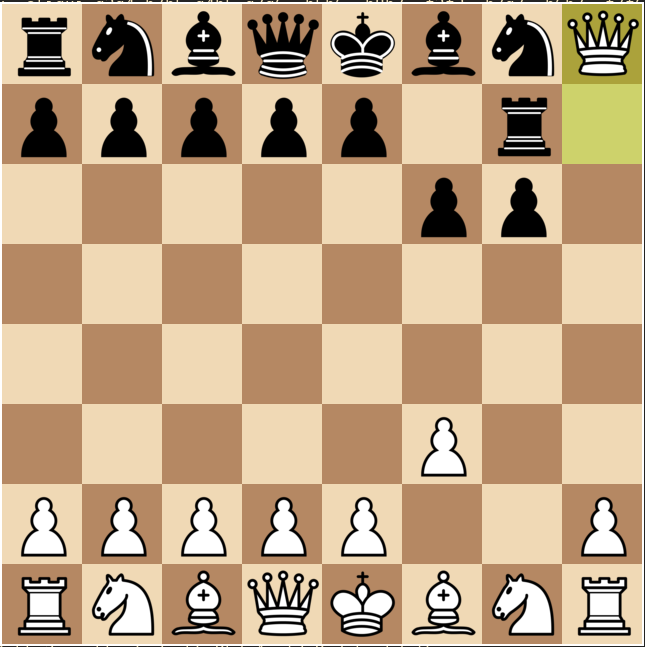
\includegraphics[scale=0.15]{{fig/promoted_pawn.png}}
    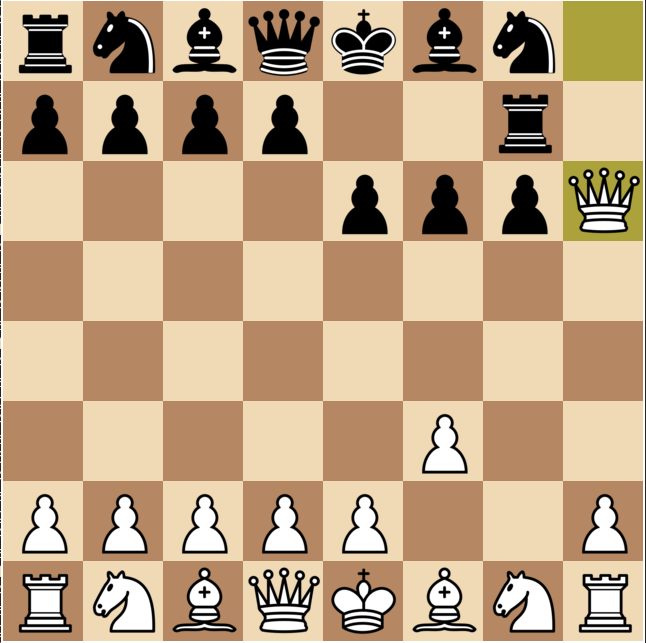
\includegraphics[scale=0.15]{{fig/queen_moving_promotion.png}}
    \caption{The most left screenshot is the result of the test, and then it was
        a sequence of screenshots of the user playing and doing the promotion
    manually.}
\end{figure}

While developing, the GUI and CLI interface could be behaving
differently, having that in mind, we can also do the same test with the CLI if we are in doubt:

\begin{lstlisting}
 >> $ python3 tests/promotionTest_cli.py
python3 chess.py -clitest g2g4 h7h5 g4h5 g7g6  h5h6  h8h7  f2f3  h7g7  h6h7  f7f6  h7h8q  e7e6 h8h6
(...)
Black's turn to move!
*********************************
8| r | n | b | q | k | b | n |   |
7| p | p | p | p |   |   | r |   |
6|   |   |   |   | p | p | p | Q |
5|   |   |   |   |   |   |   |   |
4|   |   |   |   |   |   |   |   |
3|   |   |   |   |   | P |   |   |
2| P | P | P | P | P |   |   | P |
1| R | N | B | Q | K | B | N | R |
   a   b   c   d   e   f   g   h
*********************************
    
\end{lstlisting}


\begin{lstlisting}

2022-01-16 18:11:02,057 Result of possible games with 1 ply: 20/20 - OK
2022-01-16 18:11:02,057 Elapsed time in 1 ply: 00h00m00s seconds
2022-01-16 18:11:03,073 Result of possible games with 2 ply: 400/400 - OK
2022-01-16 18:11:03,073 Elapsed time in 2 ply: 00h00m01s seconds
2022-01-16 18:11:28,139 Result of possible games with 3 ply: 8902/8902 - OK
2022-01-16 18:11:28,140 Elapsed time in 3 ply: 00h00m25s seconds
2022-01-16 18:20:02,978 Result of possible games with 4 ply: 197281/197281 - OK
2022-01-16 18:20:02,978 Elapsed time in 4 ply: 00h08m34s seconds
2022-01-16 22:00:48,487 Result of possible games with 5 ply: 4865824/4865609 - ERROR
2022-01-16 22:00:48,487 Elapsed time in 5 ply: 03h40m45s seconds
2022-01-16 22:00:48,487 Total Elapsed time: (03h49m46s)
    
\end{lstlisting}


\end{document}

